After discussing the input format and the various built-in generalization methods we can now get to the meat of the anonymization algorithm.
As Figure~\ref{fig:birds_eye_view} illustrated, the pipeline will closely resemble the steps described in the anonymization algorithm in Chapter~\ref{ch:chapter_algorithm}.

\subsection{Graph representation}

The anonymization algorithm heavily uses graphs, so we need to either implement or pick an existing graph library for Go, that can handle all the required graph operations efficiently. In this library we have chosen the latter, and selected a third-party component.

\subsubsection{Graph library requirements}

\begin{itemize}
    \setstretch{1.0}
    \item handle both directed and undirected graphs
    \item handle edge weight/cost
    \item find cycles
    \item get connected components
\end{itemize}

At the time of implementing the library, the available open source contenders were \\
\textbf{gonum}~\cite{gonum}, \textbf{yourbasic-graph}~\cite{yourbasic-graph} and \textbf{go-graph}~\cite{StepLg/go-graph}.
After briefly evaluating each library it turned out that \textbf{gonum} provides the richest feature set, supporting all of the required functions --- including topological ordering.

Gonum is a set of numeric libraries, containing libraries not only for graphs, but for matrices, statistics, linear algebra, probability distributions, network analysis and more~\cite{gonum-webpage}. In our anonymization library however we only used its graph based functionality.

\subsection{Cost graph}\label{subsec:cost_graph_algorithm}

The first step of the anonymization algorithm was to construct a cost graph. For this, we need to convert the input table into its graph based representation. Recall from Section~\ref{subsec:cost_graph_construction}, that the cost graph is a weighted full graph, where the nodes are the table rows and the edge weights between them are the generalization cost of bringing the two rows into the same partition.

The cost graph creation is handled by the \texttt{cost\_graph.go} file, while the edge weight calculation is implemented in \texttt{cost.go}.
The first part of the algorithm, creating the ``empty'' cost graph can be seen on Listing~\ref{lst:empty_cost_graph}.

\begin{figure}[H]

    \centering
    \tikzset{every picture/.style={line width=0.75pt}} %set default line width to 0.75pt

    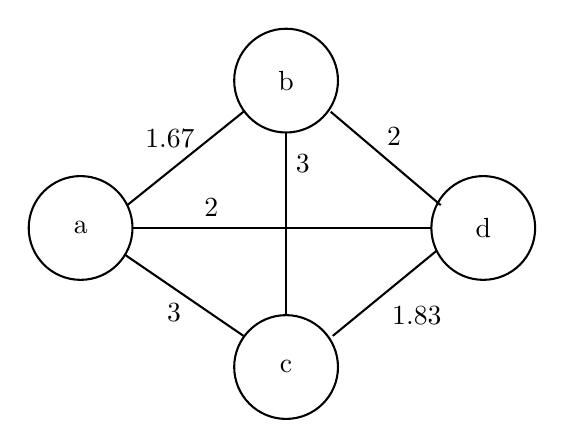
\begin{tikzpicture}[x=0.75pt,y=0.75pt,yscale=-1,xscale=1]
        %uncomment if require: \path (0,300); %set diagram left start at 0, and has height of 300

        %Shape: Circle [id:dp14719016101017623]
        \draw   (111,126) .. controls (111,112.19) and (122.19,101) .. (136,101) .. controls (149.81,101) and (161,112.19) .. (161,126) .. controls (161,139.81) and (149.81,151) .. (136,151) .. controls (122.19,151) and (111,139.81) .. (111,126) -- cycle ;
        %Shape: Circle [id:dp637969227645387]
        \draw   (210,55) .. controls (210,41.19) and (221.19,30) .. (235,30) .. controls (248.81,30) and (260,41.19) .. (260,55) .. controls (260,68.81) and (248.81,80) .. (235,80) .. controls (221.19,80) and (210,68.81) .. (210,55) -- cycle ;
        %Shape: Circle [id:dp16996306115691606]
        \draw   (210,193) .. controls (210,179.19) and (221.19,168) .. (235,168) .. controls (248.81,168) and (260,179.19) .. (260,193) .. controls (260,206.81) and (248.81,218) .. (235,218) .. controls (221.19,218) and (210,206.81) .. (210,193) -- cycle ;
        %Shape: Circle [id:dp4723269788902422]
        \draw   (305,126) .. controls (305,112.19) and (316.19,101) .. (330,101) .. controls (343.81,101) and (355,112.19) .. (355,126) .. controls (355,139.81) and (343.81,151) .. (330,151) .. controls (316.19,151) and (305,139.81) .. (305,126) -- cycle ;
        %Straight Lines [id:da43115389914855107]
        \draw    (158.5,115) -- (214.5,70) ;


        %Straight Lines [id:da3262134359528708]
        \draw    (257.5,178) -- (307.5,137) ;


        %Straight Lines [id:da6644861489456326]
        \draw    (235,168) -- (235,80) ;


        %Straight Lines [id:da44726258546505226]
        \draw    (157.5,139) -- (214.5,178) ;


        %Straight Lines [id:da17516578825824003]
        \draw    (309.5,115) -- (256.5,70) ;


        %Straight Lines [id:da25861424028019475]
        \draw    (161,126) -- (305,126) ;



        % Text Node
        \draw (136,126) node  [align=left] {a};
        % Text Node
        \draw (235,55) node  [align=left] {b};
        % Text Node
        \draw (235,193) node  [align=left] {c};
        % Text Node
        \draw (330,126) node  [align=left] {d};
        % Text Node
        \draw (179,83) node  [align=left] {1.67};
        % Text Node
        \draw (181,167) node  [align=left] {3};
        % Text Node
        \draw (199,116) node  [align=left] {2};
        % Text Node
        \draw (243,95) node  [align=left] {3};
        % Text Node
        \draw (287,82) node  [align=left] {2};
        % Text Node
        \draw (298,168) node  [align=left] {1.83};


    \end{tikzpicture}

    \caption{Example cost-graph}\label{fig:cost_graph}
\end{figure}

The code is using the \texttt{NewWeightedUndirectedGraph} function from the \emph{gonum} package. Nodes are uniquely identified with an index, which will be the number of the row they are representing in the input table.

The essence of the code that calculates edge weights can be seen on Listing~\ref{lst:cost_calculation}.

The function will try to generalize the input partitions starting from 0 to \texttt{maxLevels}, until both partitions are equal. If the two partitions are still different when generalizing them to \texttt{maxLevels} it is an error --- the Generalizer is invalid, as by definition all values should be in the same partition on the highest level.

\begin{lstlisting}[caption=Generalization cost calculation,label=lst:cost_calculation,float,floatplacement=H]
func calculateCostFraction(p1, p2 partition.Partition,
            g generalization.Generalizer) (float64, error) {
    maxLevels := g.Levels()
    for level := 0; level < maxLevels; level++ {
        g1 := g.Generalize(p1, level)
        g2 := g.Generalize(p2, level)
        if g1 != nil && g1.Equals(g2) {
            return float64(level) / float64(maxLevels-1), nil
        }
    }
    return 0, fmt.Errorf(fmt.Sprintf("data cannot be generalized
                into same partition: %v, %v", p1, p2))
}
\end{lstlisting}

\subsection{Forest building}

The forest building algorithm is responsible for constructing the directed unweighted graph, that represents the nodes (before cutting) that belong to the same partition. The algorithm is in \texttt{anon\_graph.go}. Listing~\ref{lst:forest_building} shows the outline of the algorithm.

\begin{lstlisting}[caption=Forest building algorithm,label=lst:forest_building,float,floatplacement=H]
func BuildAnonGraph(table *model.Table, k int) (graph.Directed, error) {
    costGraph, err := BuildCostGraph(table)
    if err != nil {
        return nil, err
    }
    g := buildEmptyAnonGraph(table)
    for {
        components := UndirectedConnectedComponents(g)
        c := pickComponentToExtend(components, k)
        if c == nil {
            break
        }
        u := pickSourceVertex(g, c)
        v := pickTargetVertex(g, c, u, costGraph)
        g.SetEdge(g.NewEdge(u, v))
    }
    return g, nil
}
\end{lstlisting}

The function will first build up the cost graph (see~\ref{subsec:cost_graph_algorithm}), then create an empty directed graph, which contains the nodes representing the table rows. It will then start to iterate, and picks a component to extend (based on the conditions outlined in~\ref{fig:forest_partitioning}). If there is no component to extend, the iteration has finished. Otherwise it picks a target vertex and connects the source and target vertex with a new directed edge.

\subsection{Decomposition}

The file \texttt{decompose.go} is concerned with cutting the oversized components to smaller ones, and implements all the different cut types.

The main loop of the decompose logic can be seen on Listing~\ref{lst:decompose_main}. At a high-level it is very simple: we look for a component to cut that is over the threshold, and partition it. If there is no component, we exit the loop.

\begin{lstlisting}[caption=Decompose main loop,label=lst:decompose_main,float,floatplacement=H]
func (d *Decomposer) Decompose() {
    threshold := d.getThreshold()
    for {
        c := d.pickComponent(threshold)
        if c == nil {
            break
        }
        d.partitionComponent(c)
    }
}
\end{lstlisting}

The essential part of the code for the partitioning logic is listed in~\ref{lst:decompose_partition}. After finding the \textit{u} and \textit{v} root vertices, and calculating the \textit{s} and \(\phi \) values (see Section~\ref{subsec:algorithm-to-decompose-oversized-components}) it will decide which cut type to perform. The actual implementation of the different cut types rely heavily on the gonum package and will not be listed here.

\begin{lstlisting}[caption=Partition cutting,label=lst:decompose_partition,float,floatplacement=H]
func (d *Decomposer) partitionComponent(component []graph.Node) {
    u, v, t := d.getSplitParams(component)
    s := d.calculateSize(component)
    if t >= d.k && s-t >= d.k {
        d.performCutTypeA(u, v)
    } else if s-t == d.k-1 {
        d.performCutTypeB(u, v)
    } else if t == d.k-1 {
        d.performCutTypeC(u, v)
    } else {
        d.performCutTypeD(u, v, component)
    }
}
\end{lstlisting}